% Options for packages loaded elsewhere
\PassOptionsToPackage{unicode}{hyperref}
\PassOptionsToPackage{hyphens}{url}
%
\documentclass[
  11pt,
]{article}
\usepackage{amsmath,amssymb}
\usepackage{lmodern}
\usepackage{iftex}
\ifPDFTeX
  \usepackage[T1]{fontenc}
  \usepackage[utf8]{inputenc}
  \usepackage{textcomp} % provide euro and other symbols
\else % if luatex or xetex
  \usepackage{unicode-math}
  \defaultfontfeatures{Scale=MatchLowercase}
  \defaultfontfeatures[\rmfamily]{Ligatures=TeX,Scale=1}
\fi
% Use upquote if available, for straight quotes in verbatim environments
\IfFileExists{upquote.sty}{\usepackage{upquote}}{}
\IfFileExists{microtype.sty}{% use microtype if available
  \usepackage[]{microtype}
  \UseMicrotypeSet[protrusion]{basicmath} % disable protrusion for tt fonts
}{}
\makeatletter
\@ifundefined{KOMAClassName}{% if non-KOMA class
  \IfFileExists{parskip.sty}{%
    \usepackage{parskip}
  }{% else
    \setlength{\parindent}{0pt}
    \setlength{\parskip}{6pt plus 2pt minus 1pt}}
}{% if KOMA class
  \KOMAoptions{parskip=half}}
\makeatother
\usepackage{xcolor}
\usepackage[margin=2cm]{geometry}
\usepackage{color}
\usepackage{fancyvrb}
\newcommand{\VerbBar}{|}
\newcommand{\VERB}{\Verb[commandchars=\\\{\}]}
\DefineVerbatimEnvironment{Highlighting}{Verbatim}{commandchars=\\\{\}}
% Add ',fontsize=\small' for more characters per line
\usepackage{framed}
\definecolor{shadecolor}{RGB}{248,248,248}
\newenvironment{Shaded}{\begin{snugshade}}{\end{snugshade}}
\newcommand{\AlertTok}[1]{\textcolor[rgb]{0.94,0.16,0.16}{#1}}
\newcommand{\AnnotationTok}[1]{\textcolor[rgb]{0.56,0.35,0.01}{\textbf{\textit{#1}}}}
\newcommand{\AttributeTok}[1]{\textcolor[rgb]{0.77,0.63,0.00}{#1}}
\newcommand{\BaseNTok}[1]{\textcolor[rgb]{0.00,0.00,0.81}{#1}}
\newcommand{\BuiltInTok}[1]{#1}
\newcommand{\CharTok}[1]{\textcolor[rgb]{0.31,0.60,0.02}{#1}}
\newcommand{\CommentTok}[1]{\textcolor[rgb]{0.56,0.35,0.01}{\textit{#1}}}
\newcommand{\CommentVarTok}[1]{\textcolor[rgb]{0.56,0.35,0.01}{\textbf{\textit{#1}}}}
\newcommand{\ConstantTok}[1]{\textcolor[rgb]{0.00,0.00,0.00}{#1}}
\newcommand{\ControlFlowTok}[1]{\textcolor[rgb]{0.13,0.29,0.53}{\textbf{#1}}}
\newcommand{\DataTypeTok}[1]{\textcolor[rgb]{0.13,0.29,0.53}{#1}}
\newcommand{\DecValTok}[1]{\textcolor[rgb]{0.00,0.00,0.81}{#1}}
\newcommand{\DocumentationTok}[1]{\textcolor[rgb]{0.56,0.35,0.01}{\textbf{\textit{#1}}}}
\newcommand{\ErrorTok}[1]{\textcolor[rgb]{0.64,0.00,0.00}{\textbf{#1}}}
\newcommand{\ExtensionTok}[1]{#1}
\newcommand{\FloatTok}[1]{\textcolor[rgb]{0.00,0.00,0.81}{#1}}
\newcommand{\FunctionTok}[1]{\textcolor[rgb]{0.00,0.00,0.00}{#1}}
\newcommand{\ImportTok}[1]{#1}
\newcommand{\InformationTok}[1]{\textcolor[rgb]{0.56,0.35,0.01}{\textbf{\textit{#1}}}}
\newcommand{\KeywordTok}[1]{\textcolor[rgb]{0.13,0.29,0.53}{\textbf{#1}}}
\newcommand{\NormalTok}[1]{#1}
\newcommand{\OperatorTok}[1]{\textcolor[rgb]{0.81,0.36,0.00}{\textbf{#1}}}
\newcommand{\OtherTok}[1]{\textcolor[rgb]{0.56,0.35,0.01}{#1}}
\newcommand{\PreprocessorTok}[1]{\textcolor[rgb]{0.56,0.35,0.01}{\textit{#1}}}
\newcommand{\RegionMarkerTok}[1]{#1}
\newcommand{\SpecialCharTok}[1]{\textcolor[rgb]{0.00,0.00,0.00}{#1}}
\newcommand{\SpecialStringTok}[1]{\textcolor[rgb]{0.31,0.60,0.02}{#1}}
\newcommand{\StringTok}[1]{\textcolor[rgb]{0.31,0.60,0.02}{#1}}
\newcommand{\VariableTok}[1]{\textcolor[rgb]{0.00,0.00,0.00}{#1}}
\newcommand{\VerbatimStringTok}[1]{\textcolor[rgb]{0.31,0.60,0.02}{#1}}
\newcommand{\WarningTok}[1]{\textcolor[rgb]{0.56,0.35,0.01}{\textbf{\textit{#1}}}}
\usepackage{graphicx}
\makeatletter
\def\maxwidth{\ifdim\Gin@nat@width>\linewidth\linewidth\else\Gin@nat@width\fi}
\def\maxheight{\ifdim\Gin@nat@height>\textheight\textheight\else\Gin@nat@height\fi}
\makeatother
% Scale images if necessary, so that they will not overflow the page
% margins by default, and it is still possible to overwrite the defaults
% using explicit options in \includegraphics[width, height, ...]{}
\setkeys{Gin}{width=\maxwidth,height=\maxheight,keepaspectratio}
% Set default figure placement to htbp
\makeatletter
\def\fps@figure{htbp}
\makeatother
\setlength{\emergencystretch}{3em} % prevent overfull lines
\providecommand{\tightlist}{%
  \setlength{\itemsep}{0pt}\setlength{\parskip}{0pt}}
\setcounter{secnumdepth}{-\maxdimen} % remove section numbering
% title
    \makeatletter
        \def\maketitle{%
            \pagestyle{plain}
            \begin{flushleft}
                \textsc{\small{%
                    \@author \\
                    \@date
                }}
            \end{flushleft}
            \begin{flushright}\vspace{-15mm}
            
\includegraphics[height = 1.5cm]{./files/cca.png}
            \end{flushright}
            \begin{center}\vspace{-5mm}
                \scshape{\LARGE{\scshape{Bayesian Statistics}} \\
                \normalsize \@title} \\
                \rule{0.75\linewidth}{0.1mm}
            \end{center}
            }
    \makeatother

% sections
    \usepackage{titlesec}
    \titleformat*{\section}{\Large\scshape}
    \titleformat*{\subsection}{\large\bfseries}
    \titleformat*{\subsubsection}{\normalsize\bfseries}
\newcommand{\gal}[1]{\operatorname{Galenshore}\left(#1\right)}
\newcommand{\indicator}{\mathds{1}}
\newcommand{\mean}[1]{\mathbb{E}\left[#1\right]}
\newcommand{\var}[1]{\operatorname{Var}\left(#1\right)}
\newcommand{\cov}[2]{\operatorname{Cov}\left(#1,#2\right)}
\newcommand{\corr}[2]{\operatorname{Corr}\left(#1,#2\right)}
\renewcommand{\det}[1]{\operatorname{det}\left(#1\right)}
\newcommand{\real}{\mathbb{R}}
\newcommand{\prob}[1]{\mathbb{P}\left(#1\right)}
\newcommand{\deq}{\stackrel{\text{def}}{=}}
\newcommand{\convp}{\xrightarrow{\prob}}
\renewcommand{\epsilon}{\varepsilon}
\renewcommand{\labelitemi}{\normalfont\bfseries\textendash}
\newcommand{\Gam}{\textsc{Gamma}}
\newcommand{\ssn}[2]{\operatorname{SS}\left(#1_{1:#2}\right)}
\usepackage[utf8]{inputenc}
\usepackage[T1]{fontenc}
\usepackage{dsfont}
\usepackage{cancel}
\usepackage{mathtools}
\usepackage{amsmath}
\usepackage{amsfonts}
\usepackage{amsthm}
\ifLuaTeX
  \usepackage{selnolig}  % disable illegal ligatures
\fi
\IfFileExists{bookmark.sty}{\usepackage{bookmark}}{\usepackage{hyperref}}
\IfFileExists{xurl.sty}{\usepackage{xurl}}{} % add URL line breaks if available
\urlstyle{same} % disable monospaced font for URLs
\hypersetup{
  pdftitle={Assignment 1},
  pdfauthor={Francesco Caporali, Isabel Muzio},
  hidelinks,
  pdfcreator={LaTeX via pandoc}}

\title{Assignment 1}
\author{Francesco Caporali, Isabel Muzio}
\date{24 October 2022}

\begin{document}
\maketitle

\hypertarget{question-1-the-galenshore-distribution}{%
\section{Question 1: The Galenshore
distribution}\label{question-1-the-galenshore-distribution}}

\hypertarget{point-a.}{%
\subsection{Point a.}\label{point-a.}}

\(Y | \theta \sim \operatorname{Galenshore}\left(a, \theta\right)\) is
such that \(p(y|\theta)\) is a density in the exponential family indeed
\[p(y | \theta) = \frac{2}{\Gamma(a)}\theta^{2a}y^{2a - 1}e^{-\theta^2y^2}\mathds{1}_{\left\{y > 0\right\}}, \theta > 0, a > 0.\]
Then definining \(\phi \stackrel{\text{def}}{=}\theta^2\) one has
\[p(y | \phi) = h(y)c(\phi)e^{\phi t(y)} \text{ with } h(y) =  \frac{2 y^{2a - 1}}{\Gamma(a)}\mathds{1}_{\left\{y > 0\right\}}, c(\phi) = \phi^a, t(y) = -y^2,\]
hence, by the easy shape of a distribution in the exponential family, we
can state that a class of conjugate priors for \(p(y | \phi)\) is such
that
\[p(\phi) \propto c(\phi)^{n_0}e^{\phi n_0t_0} = \phi^{a n_0}e^{\phi n_0t_0}.\]
If \(\phi\) has density \(p(\phi)\) and we want to obtain the density of
\(\theta = \sqrt{\phi}\) it is sufficient to define the map
\(f: \mathbb{R}^+ \to \mathbb{R}^+\) such that \(f(x) = \sqrt{x}\) and
recall that
\[p_{\theta}(\theta) = p_{\phi}(f(\phi)) = p_{\phi}(f^{-1}(\theta) \left|\frac{d f^{-1}(\theta)}{d \theta}\right|.\]
Observing that
\(\left|\frac{d f^{-1}(\theta)}{d \theta}\right| = \left|\frac{d \theta^2}{d \theta}\right| = 2\theta\)
\[p(\theta) \stackrel{\text{def}}{=}p_{\theta}(\theta) = p_{\phi}(\theta^2) 2 \theta \propto \theta^{2an_0} e^{\theta^2 n_0 t_0} 2 \theta.\]

\hypertarget{remark}{%
\subsubsection{Remark}\label{remark}}

Observing the three parameters \(a, n_0\) and \(t_0\) we can say

\begin{itemize}
\tightlist
\item
  \(a > 0\) by hypotesis;
\item
  \(n_0 > 0\) because it represents the \textit{prior sample size}
  (\(p(\theta)\) has the same kernel of \(p(y | \theta)\) after \(n_0\)
  observations);
\item
  \(t_0 < 0\) because it is the \textit{prior guess} that we make for
  \(t\), with
  \(t(y) = -\frac{y^2}{2}, \forall y \in \mathbb{R}^+: t_0 = \frac{\sum_{i = 1}^{n} t(y_i)}{n} = -\frac{\sum_{i = 1}^{n} y_i^2}{n} < 0\).
\end{itemize}

Hence we have \[an_0 + 1 > 0 \text{ and } -n_0t_0 > 0.\] \vspace{0.5cm}
So we can rewrite
\[p(\theta) \propto 2 \theta^{2an_0 + 1} e^{- \left(\sqrt{-n_0t_0}\right)^2 \theta^2}\]
and recognizing the kernel of a Galenshore distribution we can write
explicitly \begin{align*}
    p(\theta) & = 2 \theta^{2(an_0 + 1) - 1} e^{- \left(\sqrt{-n_0t_0}\right)^2 \theta^2} \cdot \underbrace{\frac{\left(\sqrt{-n_0t_0}\right)^{2(an_0 + 1)}}{\Gamma(an_0 + 1)}}_{\text{it does not depends on $\theta$}} \underbrace{\mathds{1}_{\theta > 0}}_{\text{by hypotesis}} = \\
    & = \frac{2}{\Gamma(an_0 + 1)} \left(\sqrt{-n_0t_0}\right)^{2(an_0 + 1)} \theta^{2(an_0 + 1) - 1} e^{- \left(\sqrt{-n_0t_0}\right)^2 \theta^2} \mathds{1}_{\theta > 0}
\end{align*} \[\Downarrow\]
\[\theta \sim \operatorname{Galenshore}\left(an_0 + 1, \sqrt{-n_0t_0}\right).\]
Finally we plot a few of these densities
\(\operatorname{Galenshore}\left(an_0 + 1, \sqrt{-n_0t_0}\right)\)
sampled with the following code:

\begin{itemize}
\tightlist
\item
  \(n_0 = 1, t_0 = -1, a = 1 \implies \operatorname{Galenshore}\left(2, 1\right)\);
\item
  \(n_0 = 2, t_0 = -1, a = 1 \implies \operatorname{Galenshore}\left(3, \sqrt{2}\right)\);
\item
  \(n_0 = 2, t_0 = -2, a = 1 \implies \operatorname{Galenshore}\left(3, 2\right)\);
\item
  \(n_0 = 2, t_0 = -2, a = 2 \implies \operatorname{Galenshore}\left(5, 2\right)\);
\item
  \(n_0 = 3, t_0 = -3, a = 1 \implies \operatorname{Galenshore}\left(4, 3\right)\);
\item
  \(n_0 = 3, t_0 = -4, a = 1 \implies \operatorname{Galenshore}\left(4, 4\right)\).
\end{itemize}

\vspace{0.5cm}

\scriptsize

\begin{Shaded}
\begin{Highlighting}[]
\NormalTok{dgalenshore }\OtherTok{=} \ControlFlowTok{function}\NormalTok{(y, a, theta) \{}
\NormalTok{    (}\DecValTok{2} \SpecialCharTok{/} \FunctionTok{gamma}\NormalTok{(a)) }\SpecialCharTok{*}\NormalTok{ theta}\SpecialCharTok{\^{}}\NormalTok{(}\DecValTok{2} \SpecialCharTok{*}\NormalTok{ a) }\SpecialCharTok{*}\NormalTok{ y}\SpecialCharTok{\^{}}\NormalTok{(}\DecValTok{2} \SpecialCharTok{*}\NormalTok{ a }\SpecialCharTok{{-}} \DecValTok{1}\NormalTok{) }\SpecialCharTok{*} \FunctionTok{exp}\NormalTok{(}\SpecialCharTok{{-}}\NormalTok{(theta}\SpecialCharTok{\^{}}\DecValTok{2}\NormalTok{) }\SpecialCharTok{*}\NormalTok{ y}\SpecialCharTok{\^{}}\DecValTok{2}\NormalTok{)}
\NormalTok{\}}

\NormalTok{y }\OtherTok{=} \FunctionTok{seq}\NormalTok{(}\FloatTok{0.01}\NormalTok{, }\FloatTok{3.5}\NormalTok{, }\AttributeTok{length =} \DecValTok{1000}\NormalTok{)}
\NormalTok{df }\OtherTok{=} \FunctionTok{rbind}\NormalTok{(}
    \FunctionTok{data.frame}\NormalTok{(}\AttributeTok{y =}\NormalTok{ y, }\AttributeTok{gal\_y =} \FunctionTok{dgalenshore}\NormalTok{(y, }\DecValTok{2}\NormalTok{, }\DecValTok{1}\NormalTok{), }\AttributeTok{label =} \StringTok{"(2, 1)"}\NormalTok{),}
    \FunctionTok{data.frame}\NormalTok{(}\AttributeTok{y =}\NormalTok{ y, }\AttributeTok{gal\_y =} \FunctionTok{dgalenshore}\NormalTok{(y, }\DecValTok{3}\NormalTok{, }\FunctionTok{sqrt}\NormalTok{(}\DecValTok{2}\NormalTok{)), }\AttributeTok{label =} \StringTok{"(3, sqrt(2))"}\NormalTok{),}
    \FunctionTok{data.frame}\NormalTok{(}\AttributeTok{y =}\NormalTok{ y, }\AttributeTok{gal\_y =} \FunctionTok{dgalenshore}\NormalTok{(y, }\DecValTok{3}\NormalTok{, }\DecValTok{2}\NormalTok{), }\AttributeTok{label =} \StringTok{"(3, 2)"}\NormalTok{),}
    \FunctionTok{data.frame}\NormalTok{(}\AttributeTok{y =}\NormalTok{ y, }\AttributeTok{gal\_y =} \FunctionTok{dgalenshore}\NormalTok{(y, }\DecValTok{5}\NormalTok{, }\DecValTok{2}\NormalTok{), }\AttributeTok{label =} \StringTok{"(5, 2)"}\NormalTok{),}
    \FunctionTok{data.frame}\NormalTok{(}\AttributeTok{y =}\NormalTok{ y, }\AttributeTok{gal\_y =} \FunctionTok{dgalenshore}\NormalTok{(y, }\DecValTok{4}\NormalTok{, }\DecValTok{3}\NormalTok{), }\AttributeTok{label =} \StringTok{"(4, 3)"}\NormalTok{),}
    \FunctionTok{data.frame}\NormalTok{(}\AttributeTok{y =}\NormalTok{ y, }\AttributeTok{gal\_y =} \FunctionTok{dgalenshore}\NormalTok{(y, }\DecValTok{4}\NormalTok{, }\DecValTok{4}\NormalTok{), }\AttributeTok{label =} \StringTok{"(4, 4)"}\NormalTok{)}
\NormalTok{)}
\end{Highlighting}
\end{Shaded}

\normalsize

Then we plot all of them at the same time: \vspace{0.5cm}

\scriptsize

\begin{Shaded}
\begin{Highlighting}[]
\FunctionTok{ggplot}\NormalTok{(df, }\FunctionTok{aes}\NormalTok{(y, gal\_y, }\AttributeTok{group =}\NormalTok{ label, }\AttributeTok{color =}\NormalTok{ label)) }\SpecialCharTok{+}
\FunctionTok{geom\_line}\NormalTok{() }\SpecialCharTok{+} \FunctionTok{coord\_fixed}\NormalTok{(}\AttributeTok{ratio =} \DecValTok{1}\NormalTok{)}
\end{Highlighting}
\end{Shaded}

\begin{center}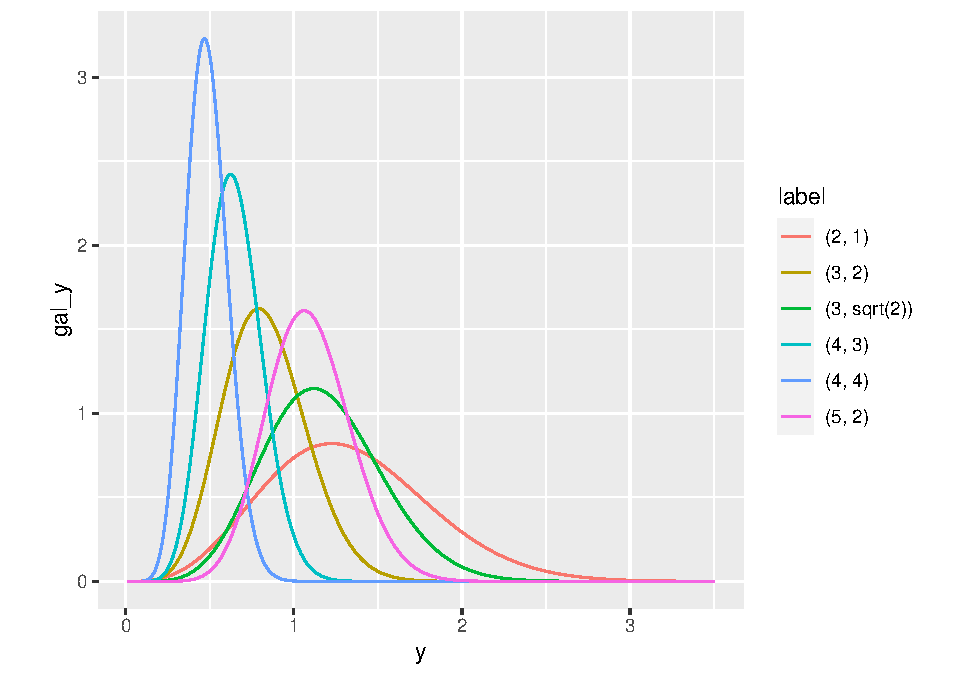
\includegraphics[width=0.6\linewidth]{1_hw_bs_code_files/figure-latex/unnamed-chunk-2-1} \end{center}
\normalsize

\hypertarget{point-b.}{%
\subsection{Point b.}\label{point-b.}}

Let's define \(b \stackrel{\text{def}}{=}an_0 + 1\) and
\(c = \sqrt{-n_0t_0}\) for coinciseness.\\
Recalling \(\theta \sim \operatorname{Galenshore}\left(b, c\right)\) and
\(Y_i | \theta \sim \operatorname{Galenshore}\left(a, \theta\right), \forall i \in 1:n\)
and defining
\(\operatorname{SS}\left(y_{1:n}\right) \stackrel{\text{def}}{=}\sum_{i = 1}^n y_i^2\)
we have \begin{align*}
    p(\theta | y_{1:n}) & = p(\theta) p(y_{1:n} | \theta) \propto \\
    & \propto (\theta^{2b - 1} e^{-c^2\theta^2}) (\theta^{2na} e^{-\theta^2\sum_{i = 1}^n y_i^2}) \propto \\
    & \propto \theta^{2(an + b) - 1} e^{-(c^2 + \operatorname{SS}\left(y_{1:n}\right))\theta^2}.
\end{align*} Hence we recognize the kernel of a
\(\operatorname{Galenshore}\left(an + b, \sqrt{c^2 + \operatorname{SS}\left(y_{1:n}\right)}\right)\)
\[\implies \theta | Y_{1:n} \sim \operatorname{Galenshore}\left(a(n + n_0) + 1, \sqrt{\operatorname{SS}\left(y_{1:n}\right) - n_0t_0}\right).\]

\hypertarget{point-c.}{%
\subsection{Point c.}\label{point-c.}}

\begin{align*}
    \frac{p(\theta_a | y_{1:n})}{p(\theta_b | y_{1:n})} & = \frac{2 \Gamma(a(n + n_0) + 1)}{\Gamma(a(n + n_0) + 1) 2}  \left(\operatorname{SS}\left(y_{1:n}\right) - n_0t_0\right)^{(a(n + n_0) + 1)(1 - 1)} \left(\frac{\theta_a}{\theta_b}\right)^{2 a(n + n_0) + 1} e^{-\left(\operatorname{SS}\left(y_{1:n}\right) - n_0t_0\right)\left(\theta_a^2 - \theta_b^2\right)} = \\
    & = \left(\frac{\theta_a}{\theta_b}\right)^{2 a(n + n_0) + 1} e^{-\left(\sum_{i = 1}^n y_i^2 - n_0t_0\right)\left(\theta_a^2 - \theta_b^2\right)}.
\end{align*} Hence
\[\mathbb{P}\left(\theta \in A | Y_{1:n} = y_{1:n}\right) = \mathbb{P}\left(\theta \in A | \sum_{i = 1}^n Y_i^2 = \sum_{i = 1}^n y_i^2\right), \forall A\]
and then, by definition
\(\operatorname{SS}\left(Y_{1:n}\right) \stackrel{\text{def}}{=}\sum_{i = 1}^n Y_i^2\)
is a sufficient statistic.

\hypertarget{point-d.}{%
\subsection{Point d.}\label{point-d.}}

Recalling that
\(\theta | Y_{1:n} \sim \operatorname{Galenshore}\left(a(n + n_0) + 1, \sqrt{\operatorname{SS}\left(y_{1:n}\right) - n_0t_0}\right)\)
and that if
\(X \sim \operatorname{Galenshore}\left(a, \theta\right) \implies \mathbb{E}\left[X\right] = \frac{\Gamma\left(a + \frac{1}{2}\right)}{\theta \Gamma(a)}\)
we have
\[\mathbb{E}\left[\theta|y_{1:n}\right] = \frac{\Gamma\left(a(n + n_0) + frac{3}{2}\right)}{\left(\sqrt{\operatorname{SS}\left(y_{1:n}\right) - n_0t_0}\right) \Gamma(a(n + n_0) + 1)}\]

\hypertarget{point-e.}{%
\subsection{Point e.}\label{point-e.}}

With the usual notation \(b \stackrel{\text{def}}{=}an_0 + 1\) and
\(c \stackrel{\text{def}}{=}\sqrt{-n_0t_0}\): \begin{align*}
    p(y_{n + 1} | y_{1:n}) & = \int_0^{\infty} p(y_{n + 1} | \theta) p(\theta | y_{1:n}) d\theta = \\
    & = \int_0^{\infty} \frac{2}{\Gamma(a)} \theta^{2a}y_{n + 1}^{2a - 1} e^{-\theta^2y_{n + 1}^2} \cdot \frac{2}{\Gamma(an + b)} \left(c^2 + \operatorname{SS}\left(y_{1:n}\right)\right)^{an + b} \theta^{2(an + b) - 1} e^{-(c^2 + \operatorname{SS}\left(y_{1:n}\right))\theta^2} d\theta =  \\
    & = \frac{4}{\Gamma(a)\Gamma(an + b)} y_{n + 1}^{2a - 1} \left(c^2 + \operatorname{SS}\left(y_{1:n}\right)\right)^{an + b} \int_0^{\infty} \underbrace{\theta^{2(a + an + b) - 1} e^{-(c^2 + \operatorname{SS}\left(y_{1:n}\right) + y_{n + 1}^2)\theta^2}}_{\text{kernel of a } \operatorname{Galenshore}\left(a + an + b, \sqrt{c^2 + \operatorname{SS}\left(y_{1:n}\right) + y_{n + 1}^2}\right)} d\theta \\
\end{align*} \[\Downarrow\] \[
    \int_0^{\infty} \theta^{2(a + an + b) - 1} e^{-(c^2 + \operatorname{SS}\left(y_{1:n}\right) + y_{n + 1}^2)\theta^2} = \frac{\Gamma(a + an + b)}{2} \left(\frac{1}{c^2 + \operatorname{SS}\left(y_{1:n}\right) + y_{n + 1}^2}\right)^{a + an + b}
\] \[\Downarrow\] \begin{align*}
    p(y_{n + 1} | y_{1:n}) & =  \frac{4}{\Gamma(a)\Gamma(an + b)} y_{n + 1}^{2a - 1} \left(c^2 + \operatorname{SS}\left(y_{1:n}\right)\right)^{an + b} \frac{\Gamma(a + an + b)}{2} \left(\frac{1}{c^2 + \operatorname{SS}\left(y_{1:n}\right) + y_{n + 1}^2}\right)^{a + an + b} = \\
    & = \frac{2}{y_{n + 1}} \frac{\Gamma(a + an + b)}{\Gamma(a)\Gamma(an + b)} \left(\frac{y_{n + 1}^2}{c^2 + \operatorname{SS}\left(y_{1:n}\right) + y_{n + 1}^2}\right)^{a} \left(\frac{c^2 + \operatorname{SS}\left(y_{1:n}\right)}{c^2 + \operatorname{SS}\left(y_{1:n}\right) + y_{n + 1}^2}\right)^{an + b} = \\
    & = \frac{2 y_{n + 1} \left(c^2 + \operatorname{SS}\left(y_{1:n}\right)\right)}{\left(c^2 + \operatorname{SS}\left(y_{1:n}\right) + y_{n + 1}^2\right)^2} \cdot \\
    & \quad \cdot \underbrace{\frac{1}{B(a, an + b)} \left(\frac{y_{n + 1}^2}{c^2 + \operatorname{SS}\left(y_{1:n}\right) + y_{n + 1}^2}\right)^{a - 1} \left(1 - \frac{y_{n + 1}^2}{c^2 + \operatorname{SS}\left(y_{1:n}\right) + y_{n + 1}^2}\right)^{(an + b) - 1}}_{\text{density of } X \sim B(a, an + b) \text{ evaluated on } \frac{y_{n + 1}^2}{c^2 + \operatorname{SS}\left(y_{1:n}\right) + y_{n + 1}^2}} = \\
    & = \frac{2 y_{n + 1} \left(c^2 + \operatorname{SS}\left(y_{1:n}\right)\right)}{\left(c^2 + \operatorname{SS}\left(y_{1:n}\right) + y_{n + 1}^2\right)^2} p_X(\frac{y_{n + 1}^2}{c^2 + \operatorname{SS}\left(y_{1:n}\right) + y_{n + 1}^2}).
\end{align*} Now one should note that this is a differentiable
transformation of \(\mathbb{R}^+\) of an unknown random variable. Indeed
if one try to derive, with respect to \(y_{n + 1}\), the variable of the
density of \(X\) in our last expression obtains \begin{align*}
    \frac{d}{d y_{n + 1}} \frac{y_{n + 1}^2}{c^2 + \operatorname{SS}\left(y_{1:n}\right) + y_{n + 1}^2} & = \frac{2y_{n + 1}(c^2 + \operatorname{SS}\left(y_{1:n}\right) + y_{n + 1}^2) - y_{n + 1}^2 2 y_{n + 1}}{\left(c^2 + \operatorname{SS}\left(y_{1:n}\right) + y_{n + 1}^2\right)^2} = \\
    & = \underbrace{\frac{2y_{n + 1}(c^2 + \operatorname{SS}\left(y_{1:n}\right))}{\left(c^2 + \operatorname{SS}\left(y_{1:n}\right) + y_{n + 1}^2\right)^2}}_{> 0 \text{ indeed $y_{n + 1} \in \mathbb{R}^+$ and the other terms are squared}}.
\end{align*} Hence if we define
\(f^{-1}: \mathbb{R}^+ \to \mathbb{R}^+\) such that
\(\displaystyle f^{-1}(x) = \frac{x^2}{c^2 + \operatorname{SS}\left(y_{1:n}\right) + x^2}\)
we can state \begin{align*}
    p(y_{n + 1} | y_{1:n}) & = \left|\frac{d}{d y_{n + 1}} f^{-1}(y_{n + 1}) \right| p_X(f^{-1}(y_{n + 1}) = \\
    & = p_{f(X)}(y_{n + 1}).
\end{align*} Let's compute \(f\) explicitly
\[f^{-1}(x) = \frac{x^2}{c^2 + \operatorname{SS}\left(y_{1:n}\right) + x^2} = 1 - \frac{c^2 + \operatorname{SS}\left(y_{1:n}\right)}{c^2 + \operatorname{SS}\left(y_{1:n}\right) + x^2}\]
hence \begin{align*}
    x = 1 - \frac{c^2 + \operatorname{SS}\left(y_{1:n}\right)}{c^2 + \operatorname{SS}\left(y_{1:n}\right) + f(x)^2} & \iff 1 - x = \frac{c^2 + \operatorname{SS}\left(y_{1:n}\right)}{c^2 + \operatorname{SS}\left(y_{1:n}\right) + f(x)^2} \iff \\
    & \iff \frac{f(x)^2}{c^2 + \operatorname{SS}\left(y_{1:n}\right)} + 1 = \frac{1}{1 - x} \iff \\
    & \iff f(x) = \sqrt{\frac{x}{1 - x}} \sqrt{c^2 + \operatorname{SS}\left(y_{1:n}\right)}.
\end{align*} This leads us to conclude (substituting again
\(b = an_0 + 1\) and \(c = \sqrt{-n_0t_0}\)) that
\[Y_{n + 1} | Y_{1:n} \sim f\left(B(a, a(n + n_0) + 1)\right), \text{ with } f: \mathbb{R}^+ \to \mathbb{R}^+, f(x) = \sqrt{\frac{x}{1 - x}} \sqrt{\operatorname{SS}\left(y_{1:n}\right) - n_0t_0}.\]

\hypertarget{question-2-tumor-counts}{%
\section{Question 2: Tumor Counts}\label{question-2-tumor-counts}}

\hypertarget{part-1-tumor-counts}{%
\subsection{Part 1: Tumor Counts}\label{part-1-tumor-counts}}

A cancer laboratory is estimating the rate of tumorigenesis in two
strains of mice, A and B. They have tumor count data for 10 mice in
strain A and 13 mice in strain B. Type A mice have been well studied,
and information from other laboratories suggests that type A mice have
tumor counts that are approximately Poisson-distributed with a mean of
12. Tumor count rates for type B mice are unknown, but type B mice are
related to type A mice.

\hypertarget{point-a.-1}{%
\subsubsection{Point a.}\label{point-a.-1}}

Given the Poisson-Gamma models defined in the problem, the posterior
distributions are: \begin{align*}
    \begin{rcases}
    Y_A \; | \; \theta_A \sim \text{Pois}(\theta_A) \\
    \theta_A \sim \text{Gamma}(120, 10)
    \end{rcases}
    & \theta_A \; | \; Y_A = \mathbf{y}_A \sim \text{Gamma}(120 + \displaystyle \sum_{i=1}^{n_A} y_{A, i} \;, 10 + n_A) \\
    \begin{rcases}
    Y_B \; | \; \theta_B \sim \text{Pois}(\theta_B) \\
    \theta_B \sim \text{Gamma}(12, 1)
    \end{rcases}
    & \theta_B \; | \; Y_B = \mathbf{y}_B \sim \text{Gamma}(12 + \displaystyle \sum_{i=1}^{n_B} y_{B, i} \;, 1 + n_B)
\end{align*} where the observed values of the samples are:
\begin{align*}
     \mathbf{y}_A = (12, 9, 12, 14, 13, 13, 15, 8, 15, 6), \quad & n_A = \text{length}(\mathbf{y}_A) \\
     \mathbf{y}_B = (11, 11, 10, 9, 9, 8, 7, 10, 6, 8, 8, 9, 7), \quad & n_B = \text{length}(\mathbf{y}_B)
\end{align*}

The consequent posterior distributions are the following:

\scriptsize

\begin{Shaded}
\begin{Highlighting}[]
\FunctionTok{load}\NormalTok{(}\AttributeTok{file =} \StringTok{\textquotesingle{}dataAssignment1.RData\textquotesingle{}}\NormalTok{)}
\FunctionTok{library}\NormalTok{(tidyverse)}
\end{Highlighting}
\end{Shaded}

\begin{verbatim}
## -- Attaching packages --------------------------------------- tidyverse 1.3.2 --
## v tibble  3.1.8      v dplyr   1.0.10
## v tidyr   1.2.1      v stringr 1.4.1 
## v readr   2.1.3      v forcats 0.5.2 
## v purrr   0.3.5      
## -- Conflicts ------------------------------------------ tidyverse_conflicts() --
## x dplyr::filter() masks stats::filter()
## x dplyr::lag()    masks stats::lag()
\end{verbatim}

\begin{Shaded}
\begin{Highlighting}[]
\FunctionTok{library}\NormalTok{(gridExtra)}
\end{Highlighting}
\end{Shaded}

\begin{verbatim}
## 
## Caricamento pacchetto: 'gridExtra'
## 
## Il seguente oggetto è mascherato da 'package:dplyr':
## 
##     combine
\end{verbatim}

\begin{Shaded}
\begin{Highlighting}[]
\FunctionTok{library}\NormalTok{(grid)}
\FunctionTok{library}\NormalTok{(ggplot2)}
\FunctionTok{library}\NormalTok{(lattice)}

\CommentTok{\#posterior parameters}

\NormalTok{a\_n }\OtherTok{=} \FloatTok{120.0} \SpecialCharTok{+} \FunctionTok{sum}\NormalTok{(y.a)}
\NormalTok{b\_n }\OtherTok{=} \FloatTok{10.0} \SpecialCharTok{+} \FunctionTok{length}\NormalTok{(y.a)}

\NormalTok{c\_n }\OtherTok{=} \DecValTok{12} \SpecialCharTok{+} \FunctionTok{sum}\NormalTok{(y.b)}
\NormalTok{d\_n }\OtherTok{=} \DecValTok{1} \SpecialCharTok{+} \FunctionTok{length}\NormalTok{(y.b)}

\FunctionTok{cat}\NormalTok{(}\FunctionTok{paste}\NormalTok{(}\StringTok{"Posterior of A : Gamma("}\NormalTok{, a\_n, }\StringTok{","}\NormalTok{, b\_n, }\StringTok{") }\SpecialCharTok{\textbackslash{}n}\StringTok{"}\NormalTok{,  }\StringTok{"Posterior of B : Gamma("}\NormalTok{, c\_n, }\StringTok{","}\NormalTok{, d\_n, }\StringTok{") }\SpecialCharTok{\textbackslash{}n}\StringTok{"}\NormalTok{))}
\end{Highlighting}
\end{Shaded}

\begin{verbatim}
## Posterior of A : Gamma( 237 , 20 ) 
##  Posterior of B : Gamma( 125 , 14 )
\end{verbatim}

\begin{Shaded}
\begin{Highlighting}[]
\CommentTok{\#posterior means}

\NormalTok{mean\_A }\OtherTok{=}\NormalTok{ a\_n }\SpecialCharTok{/}\NormalTok{ b\_n}
\NormalTok{mean\_B }\OtherTok{=}\NormalTok{ c\_n }\SpecialCharTok{/}\NormalTok{ d\_n}

\CommentTok{\#posterior densities}

\NormalTok{y.a.sum }\OtherTok{=} \FunctionTok{sum}\NormalTok{(y.a)}
\NormalTok{n.a }\OtherTok{=} \FunctionTok{length}\NormalTok{(y.a)}
\NormalTok{alpha }\OtherTok{=} \FloatTok{0.05}
\NormalTok{gamma.values }\OtherTok{=} \FunctionTok{seq}\NormalTok{(}\DecValTok{0}\NormalTok{, }\DecValTok{20}\NormalTok{, }\AttributeTok{length=} \DecValTok{200}\NormalTok{)}

\NormalTok{post.values.a }\OtherTok{=} \FunctionTok{dgamma}\NormalTok{(gamma.values, a\_n, b\_n)}
\NormalTok{post.values.b }\OtherTok{=} \FunctionTok{dgamma}\NormalTok{(gamma.values, c\_n, d\_n)}

\NormalTok{post.data }\OtherTok{=} \FunctionTok{data.frame}\NormalTok{(gamma.values, post.values.a, post.values.b)}

\CommentTok{\#posterior density plots}

\NormalTok{post.data }\SpecialCharTok{\%\textgreater{}\%} \FunctionTok{ggplot}\NormalTok{()}\SpecialCharTok{+}
  \FunctionTok{geom\_line}\NormalTok{(}\FunctionTok{aes}\NormalTok{(}\AttributeTok{x =}\NormalTok{ gamma.values, }\AttributeTok{y =}\NormalTok{ post.values.a), }\AttributeTok{col =} \StringTok{"red"}\NormalTok{, }\AttributeTok{alpha =} \FloatTok{0.6}\NormalTok{, }\AttributeTok{size =} \FloatTok{1.2}\NormalTok{)}\SpecialCharTok{+} 
  \FunctionTok{geom\_vline}\NormalTok{(}\AttributeTok{xintercept =}\NormalTok{ mean\_A, }\AttributeTok{col =} \StringTok{"red"}\NormalTok{, }\AttributeTok{linetype =} \DecValTok{2}\NormalTok{)}\SpecialCharTok{+}
  \FunctionTok{scale\_color\_discrete}\NormalTok{(}\AttributeTok{guide =} \StringTok{"none"}\NormalTok{) }\OtherTok{{-}\textgreater{}}\NormalTok{ p1}

\NormalTok{post.data }\SpecialCharTok{\%\textgreater{}\%} \FunctionTok{ggplot}\NormalTok{()}\SpecialCharTok{+}
  \FunctionTok{geom\_line}\NormalTok{(}\FunctionTok{aes}\NormalTok{(}\AttributeTok{x =}\NormalTok{ gamma.values, }\AttributeTok{y =}\NormalTok{ post.values.b), }\AttributeTok{col =} \StringTok{"blue"}\NormalTok{, }\AttributeTok{alpha =} \FloatTok{0.6}\NormalTok{, }\AttributeTok{size =} \FloatTok{1.2}\NormalTok{)}\SpecialCharTok{+}
  \FunctionTok{geom\_vline}\NormalTok{(}\AttributeTok{xintercept =}\NormalTok{ mean\_B, }\AttributeTok{col =} \StringTok{"blue"}\NormalTok{, }\AttributeTok{linetype =} \DecValTok{2}\NormalTok{)}\SpecialCharTok{+}
  \FunctionTok{scale\_color\_discrete}\NormalTok{(}\AttributeTok{guide =} \StringTok{"none"}\NormalTok{) }\OtherTok{{-}\textgreater{}}\NormalTok{ p2}

\NormalTok{p3 }\OtherTok{\textless{}{-}}\NormalTok{ p1 }\SpecialCharTok{+} 
  \FunctionTok{geom\_line}\NormalTok{(}\FunctionTok{aes}\NormalTok{(}\AttributeTok{x =}\NormalTok{ gamma.values, }\AttributeTok{y =}\NormalTok{ post.values.b), }\AttributeTok{col =} \StringTok{"blue"}\NormalTok{, }\AttributeTok{alpha =} \FloatTok{0.6}\NormalTok{, }\AttributeTok{size =} \FloatTok{1.2}\NormalTok{)}\SpecialCharTok{+}
  \FunctionTok{geom\_vline}\NormalTok{(}\AttributeTok{xintercept =}\NormalTok{ mean\_B, }\AttributeTok{col =} \StringTok{"blue"}\NormalTok{, }\AttributeTok{linetype =} \DecValTok{2}\NormalTok{)}\SpecialCharTok{+}
  \FunctionTok{xlab}\NormalTok{(}\FunctionTok{expression}\NormalTok{(theta)) }\SpecialCharTok{+}
  \FunctionTok{ylab}\NormalTok{(}\FunctionTok{expression}\NormalTok{(}\FunctionTok{paste}\NormalTok{(}\StringTok{"p("}\NormalTok{,theta,}\StringTok{"|"}\NormalTok{,y,}\StringTok{")"}\NormalTok{)))}\SpecialCharTok{+}
  \FunctionTok{ggtitle}\NormalTok{(}\StringTok{"Posterior probability densities"}\NormalTok{)  }

\NormalTok{p1 }\OtherTok{\textless{}{-}}\NormalTok{ p1 }\SpecialCharTok{+}
  \FunctionTok{xlab}\NormalTok{(}\FunctionTok{expression}\NormalTok{(theta)) }\SpecialCharTok{+}
  \FunctionTok{ylab}\NormalTok{(}\FunctionTok{expression}\NormalTok{(}\FunctionTok{paste}\NormalTok{(}\StringTok{"p("}\NormalTok{,theta[A],}\StringTok{"|"}\NormalTok{,y[A],}\StringTok{")"}\NormalTok{)))}\SpecialCharTok{+}
  \FunctionTok{ggtitle}\NormalTok{(}\FunctionTok{expression}\NormalTok{(}\FunctionTok{paste}\NormalTok{(}\StringTok{"Posterior probability density of "}\NormalTok{, theta[A])))}

\NormalTok{p2 }\OtherTok{\textless{}{-}}\NormalTok{ p2 }\SpecialCharTok{+} 
  \FunctionTok{xlab}\NormalTok{(}\FunctionTok{expression}\NormalTok{(theta)) }\SpecialCharTok{+}
  \FunctionTok{ylab}\NormalTok{(}\FunctionTok{expression}\NormalTok{(}\FunctionTok{paste}\NormalTok{(}\StringTok{"p("}\NormalTok{,theta[B],}\StringTok{"|"}\NormalTok{,y[B],}\StringTok{")"}\NormalTok{)))}\SpecialCharTok{+}
  \FunctionTok{ggtitle}\NormalTok{(}\FunctionTok{expression}\NormalTok{(}\FunctionTok{paste}\NormalTok{(}\StringTok{"Posterior probability density of "}\NormalTok{, theta[B])))}

\FunctionTok{grid.arrange}\NormalTok{(}\FunctionTok{arrangeGrob}\NormalTok{(p1, p2, }\AttributeTok{ncol =} \DecValTok{2}\NormalTok{), p3, }\AttributeTok{nrow =} \DecValTok{2}\NormalTok{)}
\end{Highlighting}
\end{Shaded}

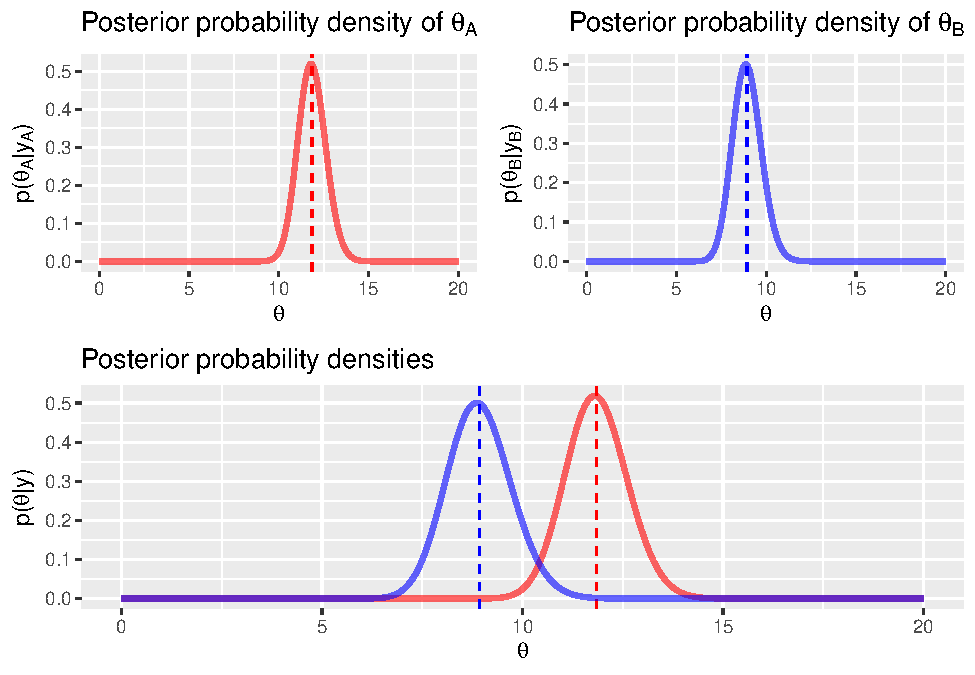
\includegraphics{1_hw_bs_code_files/figure-latex/x2a1-1.pdf}

\normalsize

Using the posterior distributions, the 95\% quantile-based intervals
are:

\scriptsize

\begin{Shaded}
\begin{Highlighting}[]
\CommentTok{\#quantile intervals}

\NormalTok{quant.interval.a }\OtherTok{=} \FunctionTok{qgamma}\NormalTok{(}\FunctionTok{c}\NormalTok{(alpha}\SpecialCharTok{/}\DecValTok{2}\NormalTok{,}\DecValTok{1}\SpecialCharTok{{-}}\NormalTok{alpha}\SpecialCharTok{/}\DecValTok{2}\NormalTok{), }\AttributeTok{shape =}\NormalTok{ a\_n, }\AttributeTok{rate =}\NormalTok{ b\_n)}
\NormalTok{quant.interval.b }\OtherTok{=} \FunctionTok{qgamma}\NormalTok{(}\FunctionTok{c}\NormalTok{(alpha}\SpecialCharTok{/}\DecValTok{2}\NormalTok{,}\DecValTok{1}\SpecialCharTok{{-}}\NormalTok{alpha}\SpecialCharTok{/}\DecValTok{2}\NormalTok{), }\AttributeTok{shape =}\NormalTok{ c\_n, }\AttributeTok{rate =}\NormalTok{ d\_n)}

\CommentTok{\#quantile{-}based intervals plots}

\NormalTok{post.data }\SpecialCharTok{\%\textgreater{}\%} \FunctionTok{ggplot}\NormalTok{()}\SpecialCharTok{+}
  \FunctionTok{geom\_line}\NormalTok{(}\FunctionTok{aes}\NormalTok{(}\AttributeTok{x =}\NormalTok{ gamma.values, }\AttributeTok{y =}\NormalTok{ post.values.a), }\AttributeTok{col=}\StringTok{"darkgreen"}\NormalTok{, }\AttributeTok{alpha =} \FloatTok{0.6}\NormalTok{, }\AttributeTok{size=}\FloatTok{1.2}\NormalTok{)}\SpecialCharTok{+}
  \FunctionTok{geom\_vline}\NormalTok{(}\AttributeTok{xintercept =}\NormalTok{ quant.interval.a[}\DecValTok{1}\NormalTok{], }\AttributeTok{col =} \StringTok{"darkgreen"}\NormalTok{)}\SpecialCharTok{+}
  \FunctionTok{geom\_vline}\NormalTok{(}\AttributeTok{xintercept =}\NormalTok{ quant.interval.a[}\DecValTok{2}\NormalTok{], }\AttributeTok{col =} \StringTok{"darkgreen"}\NormalTok{)}\SpecialCharTok{+}
  \FunctionTok{geom\_rect}\NormalTok{(}\FunctionTok{aes}\NormalTok{(}\AttributeTok{xmin =}\NormalTok{ quant.interval.a[}\DecValTok{1}\NormalTok{], }\AttributeTok{xmax =}\NormalTok{ quant.interval.a[}\DecValTok{2}\NormalTok{], }\AttributeTok{ymin =} \SpecialCharTok{{-}}\ConstantTok{Inf}\NormalTok{, }\AttributeTok{ymax =} \ConstantTok{Inf}\NormalTok{), }\AttributeTok{fill =} \StringTok{"green"}\NormalTok{, }\AttributeTok{alpha =} \FloatTok{0.002}\NormalTok{)}\SpecialCharTok{+}
  \FunctionTok{xlab}\NormalTok{(}\FunctionTok{expression}\NormalTok{(theta)) }\SpecialCharTok{+}
  \FunctionTok{ylab}\NormalTok{(}\FunctionTok{expression}\NormalTok{(}\FunctionTok{paste}\NormalTok{(}\StringTok{"p("}\NormalTok{,theta[A],}\StringTok{"|"}\NormalTok{,y[A],}\StringTok{")"}\NormalTok{)))}\SpecialCharTok{+}
  \FunctionTok{ggtitle}\NormalTok{(}\FunctionTok{expression}\NormalTok{(}\FunctionTok{paste}\NormalTok{(}\StringTok{"Quantile{-}based 95\% {-} interval of "}\NormalTok{, theta[A])))}\SpecialCharTok{+}
  \FunctionTok{scale\_color\_discrete}\NormalTok{(}\AttributeTok{guide =} \StringTok{"none"}\NormalTok{) }\OtherTok{{-}\textgreater{}}\NormalTok{q1}

\NormalTok{post.data }\SpecialCharTok{\%\textgreater{}\%} \FunctionTok{ggplot}\NormalTok{()}\SpecialCharTok{+}
  \FunctionTok{geom\_line}\NormalTok{(}\FunctionTok{aes}\NormalTok{(}\AttributeTok{x =}\NormalTok{ gamma.values, }\AttributeTok{y =}\NormalTok{ post.values.b), }\AttributeTok{col =} \StringTok{"darkorange"}\NormalTok{, }\AttributeTok{alpha =} \FloatTok{0.6}\NormalTok{, }\AttributeTok{size =} \FloatTok{1.2}\NormalTok{)}\SpecialCharTok{+} 
  \FunctionTok{geom\_vline}\NormalTok{(}\AttributeTok{xintercept =}\NormalTok{ quant.interval.b[}\DecValTok{1}\NormalTok{], }\AttributeTok{col =} \StringTok{"darkorange"}\NormalTok{)}\SpecialCharTok{+}
  \FunctionTok{geom\_vline}\NormalTok{(}\AttributeTok{xintercept =}\NormalTok{ quant.interval.b[}\DecValTok{2}\NormalTok{], }\AttributeTok{col =} \StringTok{"darkorange"}\NormalTok{)}\SpecialCharTok{+}
  \FunctionTok{geom\_rect}\NormalTok{(}\FunctionTok{aes}\NormalTok{(}\AttributeTok{xmin =}\NormalTok{ quant.interval.b[}\DecValTok{1}\NormalTok{], }\AttributeTok{xmax =}\NormalTok{ quant.interval.b[}\DecValTok{2}\NormalTok{], }\AttributeTok{ymin =} \SpecialCharTok{{-}}\ConstantTok{Inf}\NormalTok{, }\AttributeTok{ymax =} \ConstantTok{Inf}\NormalTok{), }\AttributeTok{fill =} \StringTok{"orange"}\NormalTok{, }\AttributeTok{alpha =} \FloatTok{0.002}\NormalTok{)}\SpecialCharTok{+}
  \FunctionTok{xlab}\NormalTok{(}\FunctionTok{expression}\NormalTok{(theta)) }\SpecialCharTok{+}
  \FunctionTok{ylab}\NormalTok{(}\FunctionTok{expression}\NormalTok{(}\FunctionTok{paste}\NormalTok{(}\StringTok{"p("}\NormalTok{,theta[B],}\StringTok{"|"}\NormalTok{,y[B],}\StringTok{")"}\NormalTok{)))}\SpecialCharTok{+}
  \FunctionTok{ggtitle}\NormalTok{(}\FunctionTok{expression}\NormalTok{(}\FunctionTok{paste}\NormalTok{(}\StringTok{"Quantile{-}based 95\% {-} interval of "}\NormalTok{, theta[B])))}\SpecialCharTok{+}
  \FunctionTok{scale\_color\_discrete}\NormalTok{(}\AttributeTok{guide =} \StringTok{"none"}\NormalTok{) }\OtherTok{{-}\textgreater{}}\NormalTok{ q2}


\FunctionTok{grid.arrange}\NormalTok{(q1, q2, }\AttributeTok{nrow =} \DecValTok{2}\NormalTok{)}
\end{Highlighting}
\end{Shaded}

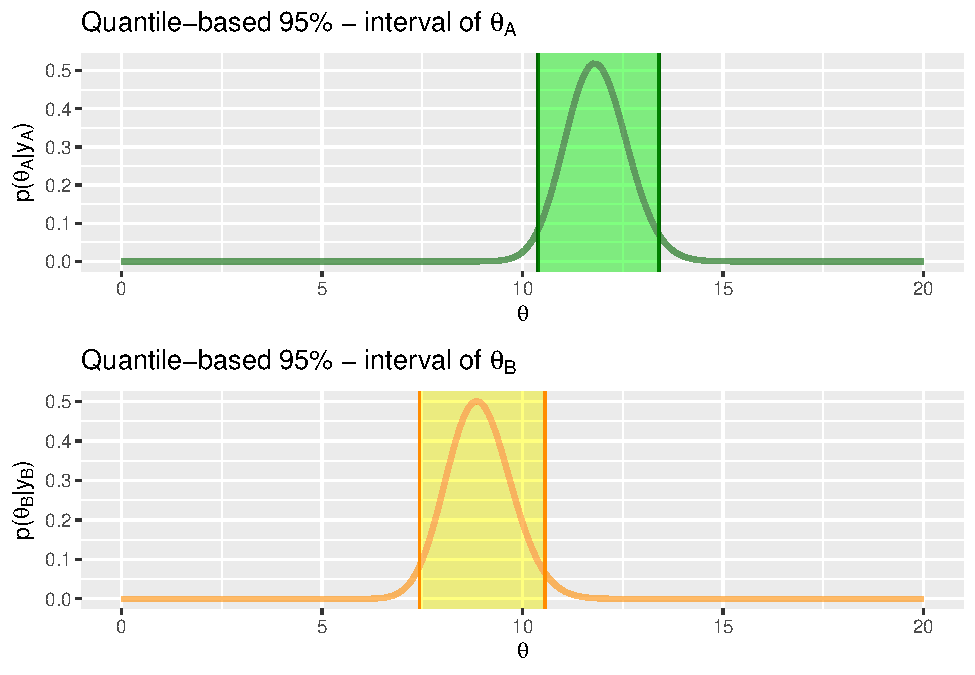
\includegraphics{1_hw_bs_code_files/figure-latex/x2a2-1.pdf} \normalsize

\hypertarget{point-b.-1}{%
\subsubsection{Point b.}\label{point-b.-1}}

Suppose we now consider a new model, where the prior for \(\theta_B\) is
dependent on a parameter \(n_0\) in the following way: \begin{align*}
    \theta_B \sim \text{Gamma}(12 x n_0, n_0})
\end{align*}

Therefore the new posterior is the following: \begin{align*}
\begin{rcases}
    Y_B \; | \; \theta_B \sim \text{Pois}(\theta_B) \\
    \theta_B \sim \text{Gamma}(12 x n_0, n_0)
    \end{rcases}
    \theta_B \; | \; Y_B = \mathbf{y}_B \sim \text{Gamma}(12 x n_0 + \displaystyle \sum_{i=1}^{n_B} y_{B, i} \;, n_0 + n_B)
\end{align*}

The posterior mean therefore depends on the parameter \(n_0\) with the
following evolution:

\scriptsize

\begin{Shaded}
\begin{Highlighting}[]
\NormalTok{mean.b }\OtherTok{=} \FunctionTok{rep}\NormalTok{(}\DecValTok{0}\NormalTok{, }\DecValTok{50}\NormalTok{)}

\NormalTok{n\_0 }\OtherTok{=} \DecValTok{1}\SpecialCharTok{:}\DecValTok{50}

\ControlFlowTok{for}\NormalTok{ (i }\ControlFlowTok{in}\NormalTok{ n\_0)\{}
\NormalTok{  a }\OtherTok{=} \DecValTok{12}\SpecialCharTok{*}\NormalTok{i }\SpecialCharTok{+} \FunctionTok{sum}\NormalTok{(y.b)}
\NormalTok{  b }\OtherTok{=}\NormalTok{ i }\SpecialCharTok{+} \FunctionTok{length}\NormalTok{(y.b)}
\NormalTok{  mean.b[i] }\OtherTok{=}\NormalTok{ a}\SpecialCharTok{/}\NormalTok{b}
\NormalTok{\}}

\NormalTok{mean\_varying }\OtherTok{\textless{}{-}} \FunctionTok{data.frame}\NormalTok{(n\_0, mean.b)}
\end{Highlighting}
\end{Shaded}

\begin{Shaded}
\begin{Highlighting}[]
\NormalTok{mean\_varying }\SpecialCharTok{\%\textgreater{}\%} \FunctionTok{ggplot}\NormalTok{(}\FunctionTok{aes}\NormalTok{(}\AttributeTok{x =}\NormalTok{ n\_0, }\AttributeTok{y =}\NormalTok{ mean.b))}\SpecialCharTok{+}
  \FunctionTok{geom\_line}\NormalTok{(}\AttributeTok{col =} \StringTok{"green4"}\NormalTok{)}\SpecialCharTok{+}
  \FunctionTok{xlab}\NormalTok{(}\FunctionTok{expression}\NormalTok{(n[}\DecValTok{0}\NormalTok{]))}\SpecialCharTok{+}
  \FunctionTok{ylab}\NormalTok{ (}\FunctionTok{expression}\NormalTok{(}\FunctionTok{paste}\NormalTok{(}\StringTok{"E["}\NormalTok{,theta[B], }\StringTok{"]"}\NormalTok{)))}\SpecialCharTok{+}
  \FunctionTok{ggtitle}\NormalTok{(}\FunctionTok{expression}\NormalTok{(}\FunctionTok{paste}\NormalTok{(}\StringTok{"Posterior mean "}\NormalTok{, }\StringTok{"E["}\NormalTok{,theta[B], }\StringTok{"]"}\NormalTok{, }\StringTok{" dependence on "}\NormalTok{, n[}\DecValTok{0}\NormalTok{])))}\SpecialCharTok{+}
  \FunctionTok{geom\_hline}\NormalTok{(}\AttributeTok{yintercept =}\NormalTok{ mean\_A, }\AttributeTok{col =} \StringTok{"red"}\NormalTok{)}\SpecialCharTok{+}
  \FunctionTok{scale\_color\_discrete}\NormalTok{(}\AttributeTok{guide =} \StringTok{"none"}\NormalTok{)}\SpecialCharTok{+}
  \FunctionTok{geom\_text}\NormalTok{(}\FunctionTok{aes}\NormalTok{(}\DecValTok{50}\NormalTok{, mean\_A, }\AttributeTok{label =}\NormalTok{ mean\_A, }\AttributeTok{vjust =} \SpecialCharTok{+}\FloatTok{1.5}\NormalTok{, }\AttributeTok{col =} \StringTok{"red"}\NormalTok{))}\SpecialCharTok{+}
  \FunctionTok{geom\_text}\NormalTok{(}\FunctionTok{aes}\NormalTok{(}\DecValTok{50}\NormalTok{, mean.b[}\DecValTok{50}\NormalTok{], }\AttributeTok{label =} \StringTok{"mean"}\NormalTok{, }\AttributeTok{vjust =} \SpecialCharTok{+}\FloatTok{1.5}\NormalTok{))}
\end{Highlighting}
\end{Shaded}

\begin{center}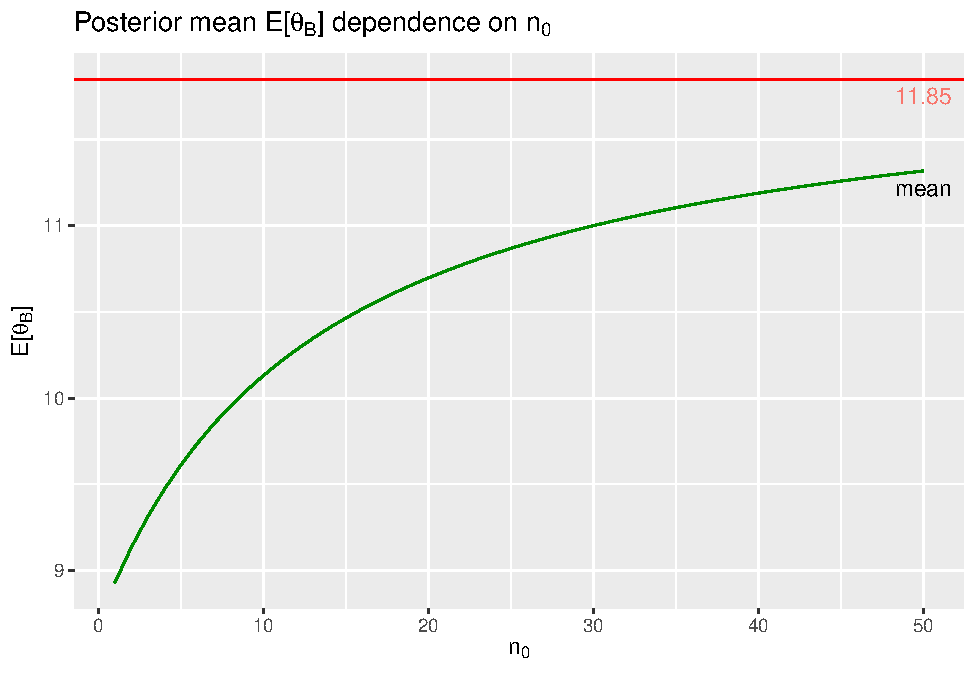
\includegraphics[width=0.6\linewidth]{1_hw_bs_code_files/figure-latex/unnamed-chunk-3-1} \end{center}
\normalsize

As we can observe, the more \(n_0\) grows, the more the posterior mean
of \(\theta_B\) approaches that of \(\theta_A\), as we can observe if we
extend the interval of variation of \(n_0\) itself:

\begin{Shaded}
\begin{Highlighting}[]
\NormalTok{mean.b }\OtherTok{=} \FunctionTok{rep}\NormalTok{(}\DecValTok{0}\NormalTok{, }\DecValTok{200}\NormalTok{)}

\NormalTok{n\_0 }\OtherTok{=} \DecValTok{1}\SpecialCharTok{:}\DecValTok{200}

\ControlFlowTok{for}\NormalTok{ (i }\ControlFlowTok{in}\NormalTok{ n\_0)\{}
\NormalTok{  a }\OtherTok{=} \DecValTok{12}\SpecialCharTok{*}\NormalTok{i }\SpecialCharTok{+} \FunctionTok{sum}\NormalTok{(y.b)}
\NormalTok{  b }\OtherTok{=}\NormalTok{ i }\SpecialCharTok{+} \FunctionTok{length}\NormalTok{(y.b)}
\NormalTok{  mean.b[i] }\OtherTok{=}\NormalTok{ a}\SpecialCharTok{/}\NormalTok{b}
\NormalTok{\}}

\NormalTok{mean\_varying\_2 }\OtherTok{\textless{}{-}} \FunctionTok{data.frame}\NormalTok{(n\_0, mean.b)}
\end{Highlighting}
\end{Shaded}

\begin{Shaded}
\begin{Highlighting}[]
\NormalTok{mean\_varying\_2 }\SpecialCharTok{\%\textgreater{}\%} \FunctionTok{ggplot}\NormalTok{(}\FunctionTok{aes}\NormalTok{(}\AttributeTok{x =}\NormalTok{ n\_0, }\AttributeTok{y =}\NormalTok{ mean.b))}\SpecialCharTok{+}
  \FunctionTok{geom\_line}\NormalTok{(}\AttributeTok{col =} \StringTok{"green4"}\NormalTok{)}\SpecialCharTok{+}
  \FunctionTok{xlab}\NormalTok{(}\FunctionTok{expression}\NormalTok{(n[}\DecValTok{0}\NormalTok{]))}\SpecialCharTok{+}
  \FunctionTok{ylab}\NormalTok{ (}\FunctionTok{expression}\NormalTok{(}\FunctionTok{paste}\NormalTok{(}\StringTok{"E["}\NormalTok{,theta[B], }\StringTok{"]"}\NormalTok{)))}\SpecialCharTok{+}
  \FunctionTok{ggtitle}\NormalTok{(}\FunctionTok{expression}\NormalTok{(}\FunctionTok{paste}\NormalTok{(}\StringTok{"Posterior mean "}\NormalTok{, }\StringTok{"E["}\NormalTok{,theta[B], }\StringTok{"]"}\NormalTok{, }\StringTok{" dependence on "}\NormalTok{, n[}\DecValTok{0}\NormalTok{])))}\SpecialCharTok{+}
  \FunctionTok{geom\_hline}\NormalTok{(}\AttributeTok{yintercept =}\NormalTok{ mean\_A, }\AttributeTok{col =} \StringTok{"red"}\NormalTok{)}\SpecialCharTok{+}
  \FunctionTok{scale\_color\_discrete}\NormalTok{(}\AttributeTok{guide =} \StringTok{"none"}\NormalTok{)}\SpecialCharTok{+}
  \FunctionTok{geom\_text}\NormalTok{(}\FunctionTok{aes}\NormalTok{(}\DecValTok{200}\NormalTok{, mean\_A, }\AttributeTok{label =}\NormalTok{ mean\_A, }\AttributeTok{vjust =} \SpecialCharTok{+}\FloatTok{1.5}\NormalTok{, }\AttributeTok{col =} \StringTok{"red"}\NormalTok{))}\SpecialCharTok{+}
  \FunctionTok{geom\_text}\NormalTok{(}\FunctionTok{aes}\NormalTok{(}\DecValTok{200}\NormalTok{, mean.b[}\DecValTok{200}\NormalTok{], }\AttributeTok{label =} \StringTok{"mean"}\NormalTok{, }\AttributeTok{vjust =} \SpecialCharTok{+}\FloatTok{1.5}\NormalTok{))}
\end{Highlighting}
\end{Shaded}

\begin{center}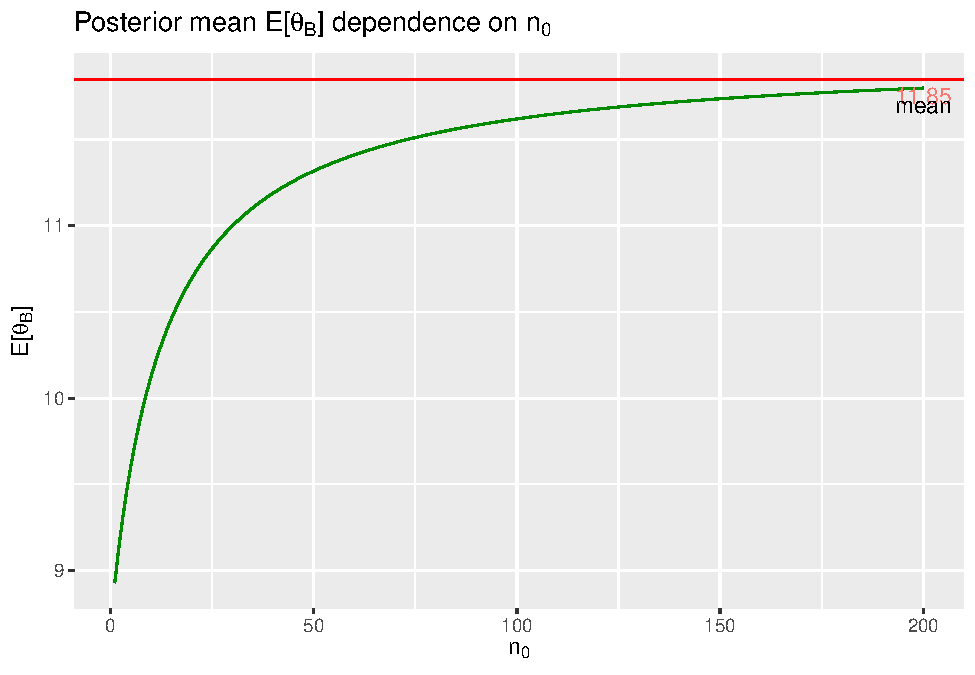
\includegraphics[width=0.6\linewidth]{1_hw_bs_code_files/figure-latex/unnamed-chunk-4-1} \end{center}

Therefore we can deduce that a large \(n_0\) is required in order to
have a posterior expectation close to that of \(\theta_A\).

\hypertarget{point-c.-1}{%
\subsubsection{Point c.}\label{point-c.-1}}

(Comments to be added)

\hypertarget{part-2-tumor-counts-comparison}{%
\subsubsection{Part 2: Tumor Counts
Comparison}\label{part-2-tumor-counts-comparison}}

\hypertarget{point-d.-1}{%
\subsubsection{Point d.}\label{point-d.-1}}

We can use the posterior distributions to obtain an approximation of
\(p \,( \, \theta_B < \theta_A \; | \; \mathbf{y}_A, \mathbf{y}_B)\)
through Monte Carlo sampling. We start by obtaining that of the original
distributions: \scriptsize

\begin{Shaded}
\begin{Highlighting}[]
\NormalTok{S }\OtherTok{=} \DecValTok{10000}

\CommentTok{\#Monte Carlo estimate with original p(theta[B])}
\NormalTok{sample.a }\OtherTok{=} \FunctionTok{rgamma}\NormalTok{(S, a\_n, b\_n)}
\NormalTok{sample.b }\OtherTok{=} \FunctionTok{rgamma}\NormalTok{(S, c\_n, d\_n)}

\NormalTok{mc1 }\OtherTok{=} \FunctionTok{sum}\NormalTok{(sample.a }\SpecialCharTok{\textgreater{}}\NormalTok{ sample.b) }\SpecialCharTok{/}\NormalTok{ S}

\FunctionTok{sprintf}\NormalTok{(}\StringTok{"The Monte Carlo estimate given the original prior of theta[B] is: \%f"}\NormalTok{, mc1)}
\end{Highlighting}
\end{Shaded}

\begin{verbatim}
## [1] "The Monte Carlo estimate given the original prior of theta[B] is: 0.996200"
\end{verbatim}

\normalsize

\hypertarget{point-e.-1}{%
\subsubsection{Point e.}\label{point-e.-1}}

Then we proceed to obtain the one for the case of the parametrized
posterior of \(\theta_B\):

\scriptsize

\begin{Shaded}
\begin{Highlighting}[]
\CommentTok{\#Monte Carlo estimate with varying p(theta[B])}
\NormalTok{n\_0 }\OtherTok{=} \DecValTok{1}\SpecialCharTok{:}\DecValTok{50}
\NormalTok{mc2 }\OtherTok{=} \FunctionTok{rep}\NormalTok{(}\DecValTok{0}\NormalTok{, }\DecValTok{50}\NormalTok{)}

\ControlFlowTok{for}\NormalTok{ (i }\ControlFlowTok{in}\NormalTok{ n\_0)\{}
\NormalTok{  a }\OtherTok{=} \DecValTok{12}\SpecialCharTok{*}\NormalTok{i }\SpecialCharTok{+} \FunctionTok{sum}\NormalTok{(y.b)}
\NormalTok{  b }\OtherTok{=}\NormalTok{ i }\SpecialCharTok{+} \FunctionTok{length}\NormalTok{(y.b)}
\NormalTok{  sample2.b }\OtherTok{=} \FunctionTok{rgamma}\NormalTok{(S, a, b)}
\NormalTok{  mc2[i] }\OtherTok{=} \FunctionTok{sum}\NormalTok{(sample.a }\SpecialCharTok{\textgreater{}}\NormalTok{ sample2.b) }\SpecialCharTok{/}\NormalTok{ S}
\NormalTok{\}}

\NormalTok{mc1\_varying }\OtherTok{\textless{}{-}} \FunctionTok{data.frame}\NormalTok{(n\_0, mc2)}
\end{Highlighting}
\end{Shaded}

\begin{Shaded}
\begin{Highlighting}[]
\NormalTok{mc1\_varying }\SpecialCharTok{\%\textgreater{}\%} \FunctionTok{ggplot}\NormalTok{(}\FunctionTok{aes}\NormalTok{(}\AttributeTok{x =}\NormalTok{ n\_0, }\AttributeTok{y =}\NormalTok{ mc2))}\SpecialCharTok{+}
  \FunctionTok{geom\_line}\NormalTok{(}\AttributeTok{col =} \StringTok{"blue"}\NormalTok{)}\SpecialCharTok{+}
  \FunctionTok{xlab}\NormalTok{(}\FunctionTok{expression}\NormalTok{(n[}\DecValTok{0}\NormalTok{]))}\SpecialCharTok{+}
  \FunctionTok{ylab}\NormalTok{ (}\FunctionTok{expression}\NormalTok{(}\FunctionTok{paste}\NormalTok{(}\StringTok{"p("}\NormalTok{,theta[A], }\StringTok{" \textgreater{} "}\NormalTok{,theta[B], }\StringTok{" | "}\NormalTok{,y[A], }\StringTok{" , "}\NormalTok{, y[B], }\StringTok{")"}\NormalTok{)))}\SpecialCharTok{+}
  \FunctionTok{ggtitle}\NormalTok{(}\FunctionTok{expression}\NormalTok{(}\FunctionTok{paste}\NormalTok{(}\StringTok{"Posterior probability dependence on "}\NormalTok{, n[}\DecValTok{0}\NormalTok{])))}\SpecialCharTok{+}
  \FunctionTok{geom\_hline}\NormalTok{(}\AttributeTok{yintercept =}\NormalTok{ mc1, }\AttributeTok{col =} \StringTok{"red"}\NormalTok{)}\SpecialCharTok{+}
  \FunctionTok{scale\_color\_discrete}\NormalTok{(}\AttributeTok{guide =} \StringTok{"none"}\NormalTok{)}\SpecialCharTok{+}
  \FunctionTok{geom\_text}\NormalTok{(}\FunctionTok{aes}\NormalTok{(}\DecValTok{50}\NormalTok{, mc1, }\AttributeTok{label =}\NormalTok{ mc1, }\AttributeTok{vjust =} \SpecialCharTok{+}\FloatTok{1.5}\NormalTok{, }\AttributeTok{col =} \StringTok{"red"}\NormalTok{))}
\end{Highlighting}
\end{Shaded}

\begin{center}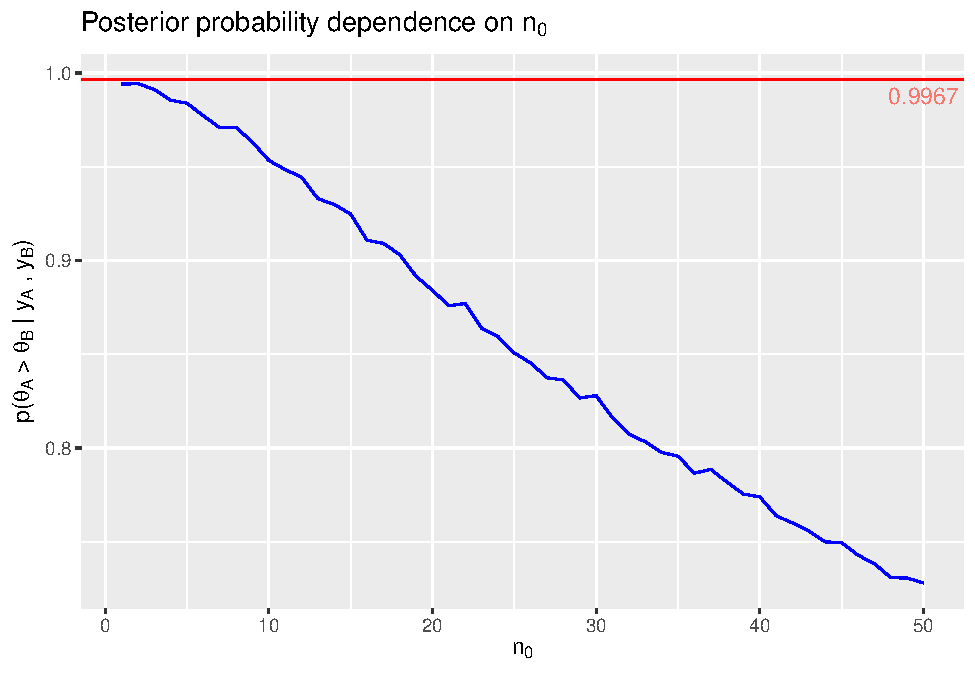
\includegraphics[width=0.6\linewidth]{1_hw_bs_code_files/figure-latex/unnamed-chunk-5-1} \end{center}
\normalsize

The resulting Monte Carlo estimate is very sensitive to the variation of
the prior of \(\theta_B\), since we have a relatively fast decay of the
probability
\(p \,( \, \theta_B < \theta_A \; | \; \mathbf{y}_A, \mathbf{y}_B)\)
with respect to the variation of the parameter \(n_0\).

\hypertarget{point-f.}{%
\subsubsection{Point f.}\label{point-f.}}

We can also obtain an estimate for
\(p \,( \, \tilde{Y_B} < \tilde{Y_A} \; | \; \mathbf{y}_A, \mathbf{y}_B)\),
where \(\tilde{Y_A}, \tilde{Y_B}\) are samples from the posterior
predictive distributions, using Monte Carlo sampling. Again we compare
the results given the original prior for \(\theta_B\) and the
parametrized one: the fall is relatively less prominent (\sim 20\%
versus \sim 40\% in the same interval of variation), but still strong,
especially considering that the starting probability was already far
lower than in the previous case.

\scriptsize

\begin{Shaded}
\begin{Highlighting}[]
\CommentTok{\#Monte Carlo estimate of the posterior predictive distribution (original theta[B])}

\NormalTok{y.post.a }\OtherTok{=} \FunctionTok{rep}\NormalTok{(}\DecValTok{0}\NormalTok{, S)}
\NormalTok{y.post.b }\OtherTok{=} \FunctionTok{rep}\NormalTok{(}\DecValTok{0}\NormalTok{, S)}

\ControlFlowTok{for}\NormalTok{ (i }\ControlFlowTok{in} \DecValTok{1}\SpecialCharTok{:}\NormalTok{S)\{}
\NormalTok{  y.post.a[i] }\OtherTok{=} \FunctionTok{rpois}\NormalTok{(}\DecValTok{1}\NormalTok{, sample.a[i])}
\NormalTok{  y.post.b[i] }\OtherTok{=} \FunctionTok{rpois}\NormalTok{(}\DecValTok{1}\NormalTok{, sample.b[i])}
\NormalTok{\}}

\NormalTok{mc3 }\OtherTok{=} \FunctionTok{sum}\NormalTok{(y.post.a }\SpecialCharTok{\textgreater{}}\NormalTok{ y.post.b)}\SpecialCharTok{/}\NormalTok{S}
\FunctionTok{sprintf}\NormalTok{(}\StringTok{"The Monte Carlo estimate given the original prior of theta[B] is: \%f"}\NormalTok{, mc3)}
\end{Highlighting}
\end{Shaded}

\begin{verbatim}
## [1] "The Monte Carlo estimate given the original prior of theta[B] is: 0.692000"
\end{verbatim}

\begin{Shaded}
\begin{Highlighting}[]
\CommentTok{\#Monte Carlo estimate of the posterior predictive distribution (varying theta[B])}

\NormalTok{mc4}\OtherTok{=} \FunctionTok{rep}\NormalTok{(}\DecValTok{0}\NormalTok{, }\DecValTok{50}\NormalTok{)}

\ControlFlowTok{for}\NormalTok{ (i }\ControlFlowTok{in} \DecValTok{1}\SpecialCharTok{:}\DecValTok{50}\NormalTok{)\{}
\NormalTok{  y.post2.b }\OtherTok{=} \FunctionTok{rep}\NormalTok{(}\DecValTok{0}\NormalTok{, S)}
\NormalTok{  a }\OtherTok{=} \DecValTok{12}\SpecialCharTok{*}\NormalTok{i }\SpecialCharTok{+} \FunctionTok{sum}\NormalTok{(y.b)}
\NormalTok{  b }\OtherTok{=}\NormalTok{ i }\SpecialCharTok{+} \FunctionTok{length}\NormalTok{(y.b)}
\NormalTok{  sample2.b }\OtherTok{=} \FunctionTok{rgamma}\NormalTok{(S, a, b)}
  \ControlFlowTok{for}\NormalTok{ (j }\ControlFlowTok{in} \DecValTok{1}\SpecialCharTok{:}\NormalTok{S)\{}
\NormalTok{  y.post2.b[j] }\OtherTok{=} \FunctionTok{rpois}\NormalTok{(}\DecValTok{1}\NormalTok{, sample2.b[j])}
\NormalTok{  \}}
\NormalTok{  mc4[i] }\OtherTok{=} \FunctionTok{sum}\NormalTok{(y.post.a }\SpecialCharTok{\textgreater{}}\NormalTok{ y.post2.b)}\SpecialCharTok{/}\NormalTok{S}
\NormalTok{\}}

\NormalTok{mc3\_varying }\OtherTok{\textless{}{-}} \FunctionTok{data.frame}\NormalTok{(n\_0, mc4)}
\end{Highlighting}
\end{Shaded}

\begin{Shaded}
\begin{Highlighting}[]
\NormalTok{mc3\_varying }\SpecialCharTok{\%\textgreater{}\%} \FunctionTok{ggplot}\NormalTok{(}\FunctionTok{aes}\NormalTok{(}\AttributeTok{x =}\NormalTok{ n\_0, }\AttributeTok{y =}\NormalTok{ mc4))}\SpecialCharTok{+}
  \FunctionTok{geom\_line}\NormalTok{(}\AttributeTok{col =} \StringTok{"darkgreen"}\NormalTok{)}\SpecialCharTok{+}
  \FunctionTok{xlab}\NormalTok{(}\FunctionTok{expression}\NormalTok{(n[}\DecValTok{0}\NormalTok{]))}\SpecialCharTok{+}
  \FunctionTok{ylab}\NormalTok{ (}\FunctionTok{expression}\NormalTok{(}\FunctionTok{paste}\NormalTok{(}\StringTok{"p("}\NormalTok{,y[A], }\StringTok{" \textgreater{} "}\NormalTok{,y[B], }\StringTok{" | "}\NormalTok{, theta[A], }\StringTok{" , "}\NormalTok{, theta[B], }\StringTok{")"}\NormalTok{)))}\SpecialCharTok{+}
  \FunctionTok{ggtitle}\NormalTok{(}\FunctionTok{expression}\NormalTok{(}\FunctionTok{paste}\NormalTok{(}\StringTok{"Posterior probability dependence on "}\NormalTok{, n[}\DecValTok{0}\NormalTok{])))}\SpecialCharTok{+}
  \FunctionTok{geom\_hline}\NormalTok{(}\AttributeTok{yintercept =}\NormalTok{ mc3, }\AttributeTok{col =} \StringTok{"darkorange"}\NormalTok{)}\SpecialCharTok{+}
  \FunctionTok{scale\_color\_discrete}\NormalTok{(}\AttributeTok{guide =} \StringTok{"none"}\NormalTok{)}\SpecialCharTok{+}
  \FunctionTok{geom\_text}\NormalTok{(}\FunctionTok{aes}\NormalTok{(}\DecValTok{50}\NormalTok{, mc3, }\AttributeTok{label =}\NormalTok{ mc3, }\AttributeTok{vjust =} \SpecialCharTok{+}\FloatTok{1.5}\NormalTok{, }\AttributeTok{col =} \StringTok{"orange"}\NormalTok{))}
\end{Highlighting}
\end{Shaded}

\begin{center}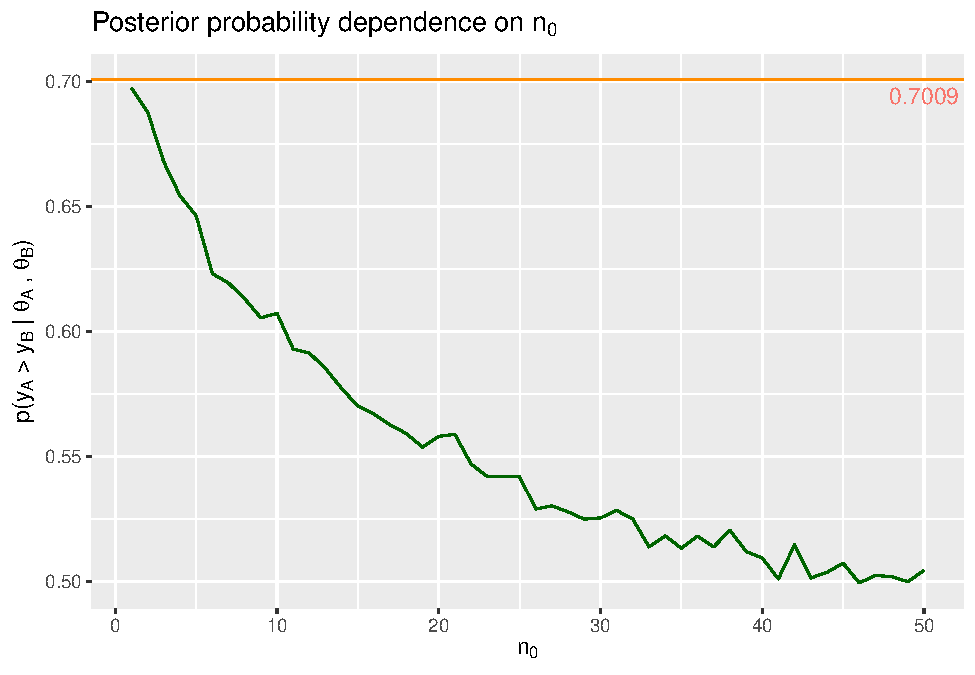
\includegraphics[width=0.6\linewidth]{1_hw_bs_code_files/figure-latex/unnamed-chunk-6-1} \end{center}
\normalsize

\hypertarget{part-3-posterior-predictive-checks}{%
\subsubsection{Part 3: Posterior predictive
checks}\label{part-3-posterior-predictive-checks}}

Lastly one can investigate the adequacy of the Poisson model for the
tumor count data in the following way.

\hypertarget{point-g.}{%
\subsubsection{Point g.}\label{point-g.}}

First we generate posterior predictive datasets
\$\mathbf{y}\^{}\{(1)\}\emph{\{A\},
\ldots{}\mathbf{y}\^{}\{(1000)\}}\{A\} \$, where each
\(\mathbf{y}^{(s)}_{A}\) is a sample of size \(n_A\) = 10 from the
Poisson distribution with parameter \(\theta^{(s)}_{A}\) and
\(\theta^{(s)}_{A}\) is itself a sample from the posterior distribution
\(p \, ( \, \theta_A \; | \; Y_A = \mathbf{y}_A)\), and \(\mathbf{y}_A\)
is the observed data.

\scriptsize

\begin{Shaded}
\begin{Highlighting}[]
\CommentTok{\#generating the samples case theta[A]}

\NormalTok{K }\OtherTok{=} \DecValTok{1000}
\NormalTok{sample.theta.a }\OtherTok{=} \FunctionTok{rgamma}\NormalTok{(K, a\_n, b\_n)}
\NormalTok{t1 }\OtherTok{=} \FunctionTok{rep}\NormalTok{(}\DecValTok{0}\NormalTok{, K)}
\ControlFlowTok{for}\NormalTok{ (i }\ControlFlowTok{in} \DecValTok{1}\SpecialCharTok{:}\NormalTok{K)\{}
\NormalTok{  post.pred.a }\OtherTok{=} \FunctionTok{rpois}\NormalTok{(}\DecValTok{10}\NormalTok{, sample.theta.a[i])}
\NormalTok{  t1[i] }\OtherTok{=} \FunctionTok{sum}\NormalTok{(post.pred.a) }\SpecialCharTok{/}\NormalTok{ (}\DecValTok{10}\SpecialCharTok{*}\FunctionTok{sd}\NormalTok{(post.pred.a))}
\NormalTok{\}}

\NormalTok{t2 }\OtherTok{=}  \FunctionTok{sum}\NormalTok{(y.a) }\SpecialCharTok{/}\NormalTok{ (}\DecValTok{10}\SpecialCharTok{*}\FunctionTok{sd}\NormalTok{(y.a))}

\NormalTok{t.a }\OtherTok{\textless{}{-}} \FunctionTok{data.frame}\NormalTok{(}\DecValTok{1}\SpecialCharTok{:}\NormalTok{K, t1)}

\NormalTok{colors }\OtherTok{\textless{}{-}} \FunctionTok{c}\NormalTok{(}\StringTok{"data mean"} \OtherTok{=} \StringTok{"blue"}\NormalTok{, }\StringTok{"sample mean"} \OtherTok{=} \StringTok{"red"}\NormalTok{)}
\end{Highlighting}
\end{Shaded}

\begin{Shaded}
\begin{Highlighting}[]
\NormalTok{t.a }\SpecialCharTok{\%\textgreater{}\%} \FunctionTok{ggplot}\NormalTok{()}\SpecialCharTok{+}
  \FunctionTok{geom\_histogram}\NormalTok{(}\FunctionTok{aes}\NormalTok{(t1), }\AttributeTok{bins =} \DecValTok{50}\NormalTok{, }\AttributeTok{fill =} \StringTok{"darkorchid"}\NormalTok{, }\AttributeTok{alpha =} \FloatTok{0.6}\NormalTok{, }\AttributeTok{col =} \StringTok{"grey"}\NormalTok{)}\SpecialCharTok{+}
  \FunctionTok{geom\_vline}\NormalTok{(}\FunctionTok{aes}\NormalTok{(}\AttributeTok{xintercept =}\NormalTok{ t2, }\AttributeTok{col =} \StringTok{"sample mean"}\NormalTok{), }\AttributeTok{size =} \FloatTok{1.2}\NormalTok{) }\SpecialCharTok{+}
  \FunctionTok{geom\_vline}\NormalTok{(}\FunctionTok{aes}\NormalTok{( }\AttributeTok{xintercept =} \FunctionTok{mean}\NormalTok{(t1), }\AttributeTok{col =} \StringTok{"data mean"}\NormalTok{), }\AttributeTok{size =} \FloatTok{1.2}\NormalTok{)}\SpecialCharTok{+}
  \FunctionTok{scale\_color\_manual}\NormalTok{(}\AttributeTok{name =} \StringTok{"Legend"}\NormalTok{, }\AttributeTok{values =} \FunctionTok{c}\NormalTok{( }\StringTok{"sample mean"} \OtherTok{=} \StringTok{"blue"}\NormalTok{, }\StringTok{"data mean"} \OtherTok{=} \StringTok{"red"}\NormalTok{),}
    \AttributeTok{labels =} \FunctionTok{c}\NormalTok{(}\StringTok{"sample mean"}\NormalTok{, }\StringTok{"data mean"}\NormalTok{))}
\end{Highlighting}
\end{Shaded}

\begin{center}\includegraphics[width=0.6\linewidth]{1_hw_bs_code_files/figure-latex/unnamed-chunk-7-1} \end{center}
\normalsize

We can see that while the distribution is very spread out, the expected
value of the statistic is close to the one observed from the data.
(comments)

\hypertarget{point-h.}{%
\subsubsection{Point h.}\label{point-h.}}

We can repeat the same procedure with the second model, by generting
posterior predictive datasets \$\mathbf{y}\^{}\{(1)\}\emph{\{B\},
\ldots{}\mathbf{y}\^{}\{(1000)\}}\{B\} \$, where each
\(\mathbf{y}^{(s)}_{B}\) is a sample of size \(n_B\) = 13 from the
Poisson distribution with parameter \(\theta^{(s)}_{B}\) and
\(\theta^{(s)}_{B}\) is itself a sample from the posterior distribution
\(p \, ( \, \theta_B \; | \; Y_B = \mathbf{y}_B)\), and \(\mathbf{y}_B\)
is the observed data. \scriptsize

\begin{Shaded}
\begin{Highlighting}[]
\CommentTok{\#generating the samples case theta[B]}

\NormalTok{K }\OtherTok{=} \DecValTok{1000}
\NormalTok{sample.theta.b }\OtherTok{=} \FunctionTok{rgamma}\NormalTok{(K, c\_n, d\_n)}
\NormalTok{t3 }\OtherTok{=} \FunctionTok{rep}\NormalTok{(}\DecValTok{0}\NormalTok{, K)}
\ControlFlowTok{for}\NormalTok{ (i }\ControlFlowTok{in} \DecValTok{1}\SpecialCharTok{:}\NormalTok{K)\{}
\NormalTok{  post.pred.b }\OtherTok{=} \FunctionTok{rpois}\NormalTok{(}\DecValTok{13}\NormalTok{, sample.theta.b[i])}
\NormalTok{  t3[i] }\OtherTok{=} \FunctionTok{sum}\NormalTok{(post.pred.a) }\SpecialCharTok{/}\NormalTok{ (}\DecValTok{13}\SpecialCharTok{*}\FunctionTok{sd}\NormalTok{(post.pred.b))}
\NormalTok{\}}

\NormalTok{t4 }\OtherTok{=}  \FunctionTok{sum}\NormalTok{(y.a) }\SpecialCharTok{/}\NormalTok{ (}\DecValTok{13}\SpecialCharTok{*}\FunctionTok{sd}\NormalTok{(y.a))}

\NormalTok{t.b }\OtherTok{\textless{}{-}} \FunctionTok{data.frame}\NormalTok{(}\DecValTok{1}\SpecialCharTok{:}\NormalTok{K, t3)}
\end{Highlighting}
\end{Shaded}

\begin{Shaded}
\begin{Highlighting}[]
\NormalTok{t.b }\SpecialCharTok{\%\textgreater{}\%} \FunctionTok{ggplot}\NormalTok{()}\SpecialCharTok{+}
  \FunctionTok{geom\_histogram}\NormalTok{(}\FunctionTok{aes}\NormalTok{(t3), }\AttributeTok{bins =} \DecValTok{50}\NormalTok{, }\AttributeTok{fill =} \StringTok{"darkorchid"}\NormalTok{, }\AttributeTok{alpha =} \FloatTok{0.6}\NormalTok{, }\AttributeTok{col =} \StringTok{"grey"}\NormalTok{)}\SpecialCharTok{+}
  \FunctionTok{geom\_vline}\NormalTok{(}\FunctionTok{aes}\NormalTok{(}\AttributeTok{xintercept =}\NormalTok{ t4, }\AttributeTok{col =} \StringTok{"sample mean"}\NormalTok{), }\AttributeTok{size =} \FloatTok{1.2}\NormalTok{) }\SpecialCharTok{+}
  \FunctionTok{geom\_vline}\NormalTok{(}\FunctionTok{aes}\NormalTok{( }\AttributeTok{xintercept =} \FunctionTok{mean}\NormalTok{(t3), }\AttributeTok{col =} \StringTok{"data mean"}\NormalTok{), }\AttributeTok{size =} \FloatTok{1.2}\NormalTok{)}\SpecialCharTok{+}
  \FunctionTok{scale\_color\_manual}\NormalTok{(}\AttributeTok{name =} \StringTok{"Legend"}\NormalTok{, }\AttributeTok{values =} \FunctionTok{c}\NormalTok{( }\StringTok{"sample mean"} \OtherTok{=} \StringTok{"blue"}\NormalTok{, }\StringTok{"data mean"} \OtherTok{=} \StringTok{"red"}\NormalTok{),}
    \AttributeTok{labels =} \FunctionTok{c}\NormalTok{(}\StringTok{"sample mean"}\NormalTok{, }\StringTok{"data mean"}\NormalTok{))}
\end{Highlighting}
\end{Shaded}

\begin{center}\includegraphics[width=0.6\linewidth]{1_hw_bs_code_files/figure-latex/unnamed-chunk-8-1} \end{center}
\normalsize

\end{document}
